\capitulo{5}{Aspectos relevantes del desarrollo del proyecto} \label{cap:aspectos}
Realizar un videojuego es un proceso largo y costoso, con numerosos factores que influyen en la rapidez y dificultad de poder desarrollar e implementar correctamente todas las funciones y requisitos deseados.

Gracias a los recursos \textit{online} disponibles, entre ellos la propia documentación de Unity, se ha podido llevar a cabo determinadas resoluciones, así como las propias planteadas para el proyecto. Por ello, en este apartado se explica en profundidad los aspectos clave del desarrollo del proyecto, entre ellos los problemas surgidos y la manera de solventarlos.

\section{Inicio del proyecto}

El 10 de marzo de 2020 se inauguró oficialmente la actividad de ÍTACA (Centro en Innovación y Tecnología de Videojuegos y Comunicación Audiovisual) en la Universidad de Burgos, cuya finalidad es desarrollar iniciativas y actividades de investigación, docencia y emprendimiento universitario en el ámbito de la industria de los videojuegos y otras nuevas tecnologías de la comunicación audiovisual \cite{itaca}.

Este centro ofertó la posibilidad de realizar un Trabajo de Fin de Grado con ellos en forma de videojuego. Una estudiante del curso pasado, Claudia Calvo Cuetos, realizó un Trabajo de Fin de Grado relacionado con una idea a futuro de realizar un videojuego de carreras divulgativo con mujeres ingenieras como protagonistas \cite{itaca:tfg}. 

Fue este llamativo conjunto de ideas y forma la motivación para escogerlo como trabajo, pues el ámbito de los videojuegos siempre ha sido algo muy atractivo y poder indagar en profundidad en este campo podía ser muy apasionante.

Escogido el proyecto y el motor de videojuego en el cual se realizaría, y una vez se acordó quiénes lo tutorizarían, se procedió a comenzar la organización del proyecto.

Al tratarse de un proyecto multidisciplinar en el cual se ha participado por parte de Ingeniería Informática y por parte de ÍTACA, donde se han visto involucrados otros Trabajos de Fin de Grado/Máster en el proyecto, primeramente, se mantuvieron varias reuniones de toma de contacto y para organizar las tareas a lo largo de las semanas.

Inicialmente, debido al desconocimiento de este motor, se dedicaron los primeros meses a la investigación para aprender a entenderlo y usarlo. Una vez se comprendieron las bases, se dio comienzo al desarrollo.

\section{Metodología de desarrollo Kanban}

Al tratarse de un proyecto en el cual el flujo de trabajo es continuo, la metodología que se ha seguido ha sido Kanban. Permite realizar las tareas a medida que van surgiendo y acabándolas según la importancia que tengan. Además, es una metodología más flexible que otras existentes actualmente, lo que ha permitido poder dedicar tiempo a investigar sobre el funcionamiento de las herramientas, ya que en el caso de usar otra metodología con ciclos predefinidos habría imposibilitado el correcto cumplimiento de las fechas.

El funcionamiento ha sido explicado en el capítulo 4 \hyperref[cap:tecnicas]{``Técnicas y Herramientas''}. Aplicándolo a este proyecto, ha permitido tener un margen de aprendizaje sobre el funcionamiento de Unity, incluyendo las pruebas realizadas con modelos, componentes y otros elementos.

Este flujo de trabajo permite, además, ajustar en el futuro las estimaciones que se hagan respecto a nuevas tareas similares y tomar este histórico de valores como referencia para el coste de cuánto supondría, ayudando también a que usuarios de otros proyectos similares no tengan que obtener datos, sino que ya pueda partir de estas mediciones para saber cuánto tiempo puede conllevar realizarlas.

Gracias a esta metodología de desarrollo, se ha podido mantener un ritmo de trabajo constante, así como ha permitido realizar las paradas necesarias para asimilar nuevos conceptos, corregir fallos y reformular la forma de completar las tareas, de manera que la presión en base al tiempo, teniendo en cuenta el contexto, ha sido menor y se ha podido llevar a cabo de una manera más fluida.

De igual forma, sí que se llevaron a cabo \textit{sprints}, de una duración de aproximadamente dos semanas por \textit{sprint} para ir llevando el control mencionado atrás del número tareas completadas y el cambio de fases.

\section{Formación}

Dado que al principio del proyecto había desconocimiento sobre el funcionamiento de Unity, se requirió de documentación externa para obtener los conocimientos necesarios para la realización correcta del proyecto.

Inicialmente se recurrió a recursos tutoriales en forma de vídeo adjuntados por el tutor, donde previamente explicaba los principios básicos de funcionamiento de Unity, así como sus elementos principales y el funcionamiento. Términos como ``transformada'', ``\textit{GameObject}'', ``\textit{Quaternion}'', ``componente'', ``asset'' o ``prefab'' entre otros, cuyo conocimiento previo sobre ellos era nulo, sentaron las primeras bases para poder empezar a hacer pruebas en el motor.

Una vez comenzó el desarrollo se recurrió a la misma documentación de Unity para comprender la utilidad y el \textit{manejo} de determinadas funciones del motor por código, así como a más recursos tutoriales en forma de vídeo respecto a la creación ciertos métodos, de los cuales se obtenía la forma de realizarlo y luego se integraba en base a la necesidad en el proyecto, dando muchos casos en los que la creación de los métodos partía totalmente de cero y otros en los que se dio la necesidad de refactorizar y adaptar.

\section{Desarrollo del proyecto}

Como se ha comentado previamente, los primeros meses fueron de formación, aunque durante el desarrollo requiriese también de cierto aprendizaje respecto a nuevos conceptos y herramientas, por lo que comenzó algo más tardío el \textit{arranque} del mismo.

Para explicar las fases de desarrollo, se dividirá en tres fases correspondientes a las versiones del proyecto: \textit{alpha}, \textit{beta} y \textit{Release candidates}.

\subsubsection{Alpha}

Inicialmente, se comenzó creando un escenario de pruebas simple conformado por dos planos, siendo estos dos objetos de tipo cubo con el grosor mínimo para obtener la forma aplanada, y ensanchados y alargados, siendo uno de ellos algo menor de tamaño que el otro para hacer superficie sobre superficie. De esta manera, se obtenía un pequeño desnivel por el que, a continuación, bajo un modelo de vehículo simple hecho a partir de cilindros como cuerpo y ruedas, se realizaban las pruebas.

Este modelo de vehículo simple, por sí mismo, no tiene utilidad, pues es solo un cuerpo ``inerte''. Ahí es donde comenzaron los primeros pasos grandes con la programación. Debido a que un sistema de conducción básico es relativamente complejo, se decidió partir de uno ya existente a partir del cual se iba a refactorizar las nuevas funciones a implementar en caso de ser necesario con el mismo, además de la creación de un sistema de cámara en tercera persona básico. Las pruebas que se hicieron al respecto llevaban a ver cómo el vehículo tenía comportamientos no esperados con el componente añadido para la conducción, con vibraciones no deseadas y otros aspectos. Hubo que realizar cambios en la configuración del componente hasta tenerlo en un estado aceptable, pero tampoco se indagó mucho en ello, pues seguía siendo un escenario de pruebas y no era rentable esforzarse en hacer cambios grandes si no iban a ser el escenario y vehículo finales.

Más adelante, se obtuvo un escenario de pruebas similar al escenario final en estructura adjuntado por el equipo de ÍTACA, de manera que ahí se podía ir realizando cambios en la configuración mencionada del vehículo previo respecto al escenario. 

En este escenario se empezaron a integrar los sistemas que componen un juego de carreras contrarreloj. Primero se creó un controlador de carrera encargado de instanciar los vehículos en la escena. Este controlador iría en un objeto al cual se llamaría de la misma manera para tener un control correcto de todos los componentes de la escena, sistema de nomenclatura que se seguiría de ahí en adelante. 

Antes de continuar con los componentes de carrera contrarreloj, se sustituyó la cámara básica por \textit{Cinemachine}, el cual es un \textit{package} gratuito descargable desde Unity, aportando un sistema de cámaras dinámico, configurable y con más realismo, fluyendo con el movimiento del vehículo y siendo más agradable que una cámara estática fija.

El siguiente elemento básico que se desarrolló fue el sistema de puntos de control, con el cual se podría crear más adelante un conteo de vueltas y un sistema de recolocación. Aprovechando los objetos que provee Unity como son los cubos, se hicieron planos en los cuales se introducían los componentes correspondientes a los puntos de control, los cuales fueron creados por código. Inicialmente eran componentes individuales, pero más adelante se cambió el sistema para que fuese el controlador de carrera el encargado.

Con el sistema creado se podía proceder a la creación del sistema de \textit{respawn} o recolocación del vehículo (manual y automático), donde gracias a ello se puede recolocar el vehículo en caso de volcar, caer fuera del escenario u otras ocasiones en las cuales no se puede realizar ningún tipo de movimiento con el vehículo, y el conteo de vueltas para que tenga un final la partida. Entre medias también se creó un cronómetro de tiempo, el cual serviría para obtener el mejor tiempo realizado en la carrera mediante la creación de otro componente. Con estos elementos creados se tenía el principal funcionamiento de una contrarreloj.

Para el último \textit{sprint} antes de la beta se ``pulieron'' todas las funciones, refactorizaron métodos, actualizado el mapa a una versión mejorada e incluidas nuevas funcionalidades, entre ellos la creación de una cuenta atrás (con el correspondiente bloqueo de vehículo previo a comenzar que conlleva), la posibilidad de acabar la carrera una vez acaben las vueltas y la creación de los menús (incluido el de pausa de partida).

\subsubsection{Beta}

Es la fase previa a la versión candidata a ser publicada. En esta fase se realizó una ``limpieza'' de componentes innecesarios en la escena, recolocación de \textit{assets}, se corrigieron \textit{bugs} varios y se cambió la lógica de algunas funciones como el conteo de puntos de control, el sistema de recolocación y el cálculo del mejor tiempo por vuelta.

Lo más destacable en esta fase es el comprobar cómo el desarrollo de las funciones tenía una cierta complejidad, pero que es a la hora de perfeccionar, corregir y cambiar la lógica de las funciones cuando aumenta esta complejidad y se hace denotar.

\subsubsection{Release candidates}

En este último \textit{sprint} se ha actualizado el modelo de vehículo, el mapa a una versión mejorada visual y estructuralmente, así como la redacción final de la documentación.

Es la versión candidata a ser publicada como juego final en el TFG, con la \textit{build} correspondiente lista para probar y jugar.

\begin{figure}[h]
	\centering
	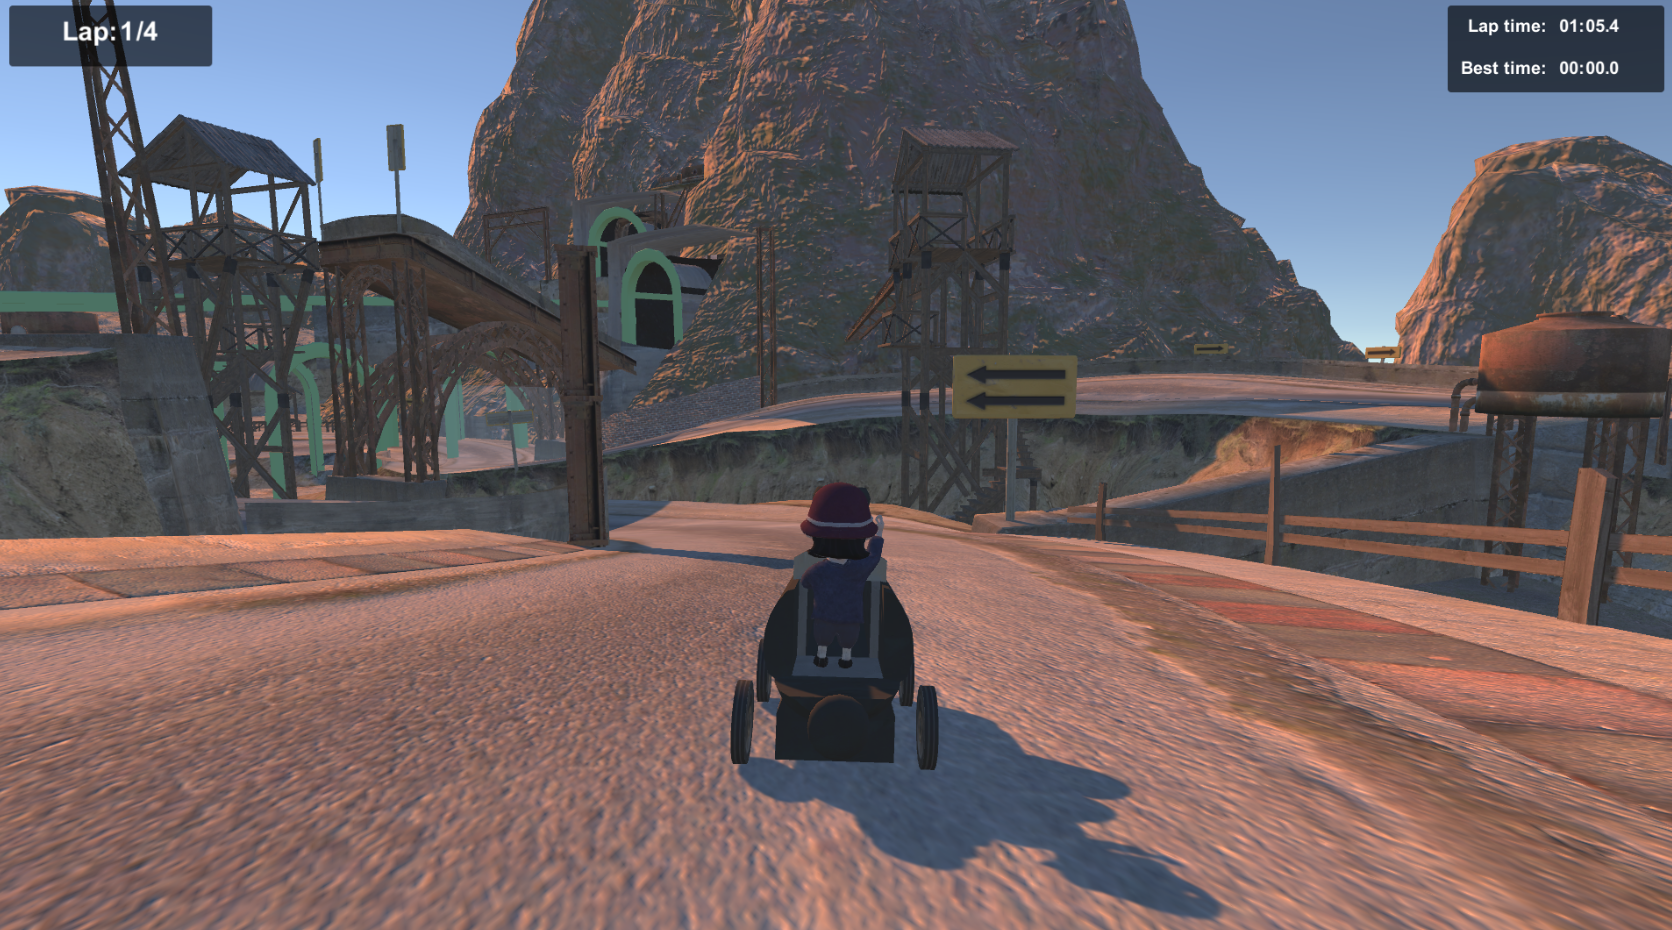
\includegraphics[width=\textwidth]{releasecandidate}
	\caption{Fotograma de la \textit{Release Candidate 1} de ``Fastastic Roads''.}
	\label{fig:releasecandidate}
\end{figure}

\subsection{Desarrollo coordinado en un equipo multidisciplinar}

Uno de los puntos destacables de este proyecto es el haber trabajado formando parte de un equipo multidisciplinar, pues se ha tenido que hacer en conjunto a un equipo de personas dedicadas a otros aspectos del juego, como han sido el escenario y los modelos 3D, así como la idea principal del juego.

Ha habido constante comunicación respecto a dudas, problemas que pudiesen surgir o necesidades momentáneas, así como reuniones cada al menos dos semanas para actualizar el progreso de cada miembro del equipo y mandar nuevas tareas en base a ese avance.

\subsubsection{Narrativa}

Aunque la narrativa está prácticamente ausente, no carece de importancia, pues la idea principal aportada por el equipo es el mostrar históricamente la implicación de los personajes en los vehículos que manejan, aportando unas características especiales que el resto de vehículos no tienen. Debido al tamaño del proyecto, se tuvo que simplificar esta idea en un juego más simple con modo a contrarreloj, teniendo la intención de continuarlo más adelante.

\subsubsection{Arte}

Para la parte artística, el resto del equipo ha sido el encargado de crear los modelos 3D para los vehículos, escenarios y animaciones bajo el software de código abierto \textit{Blender}. Estos modelos se insertaban en Unity directamente, haciendo el mismo motor la debida importación, y en ocasiones se ha tenido que exportar a formato ``.fbx'' (\textit{Filmbox}) para determinadas configuraciones, pero en general han sido en el mismo formato \textit{Blender}.

\begin{figure}[h]
	\centering
	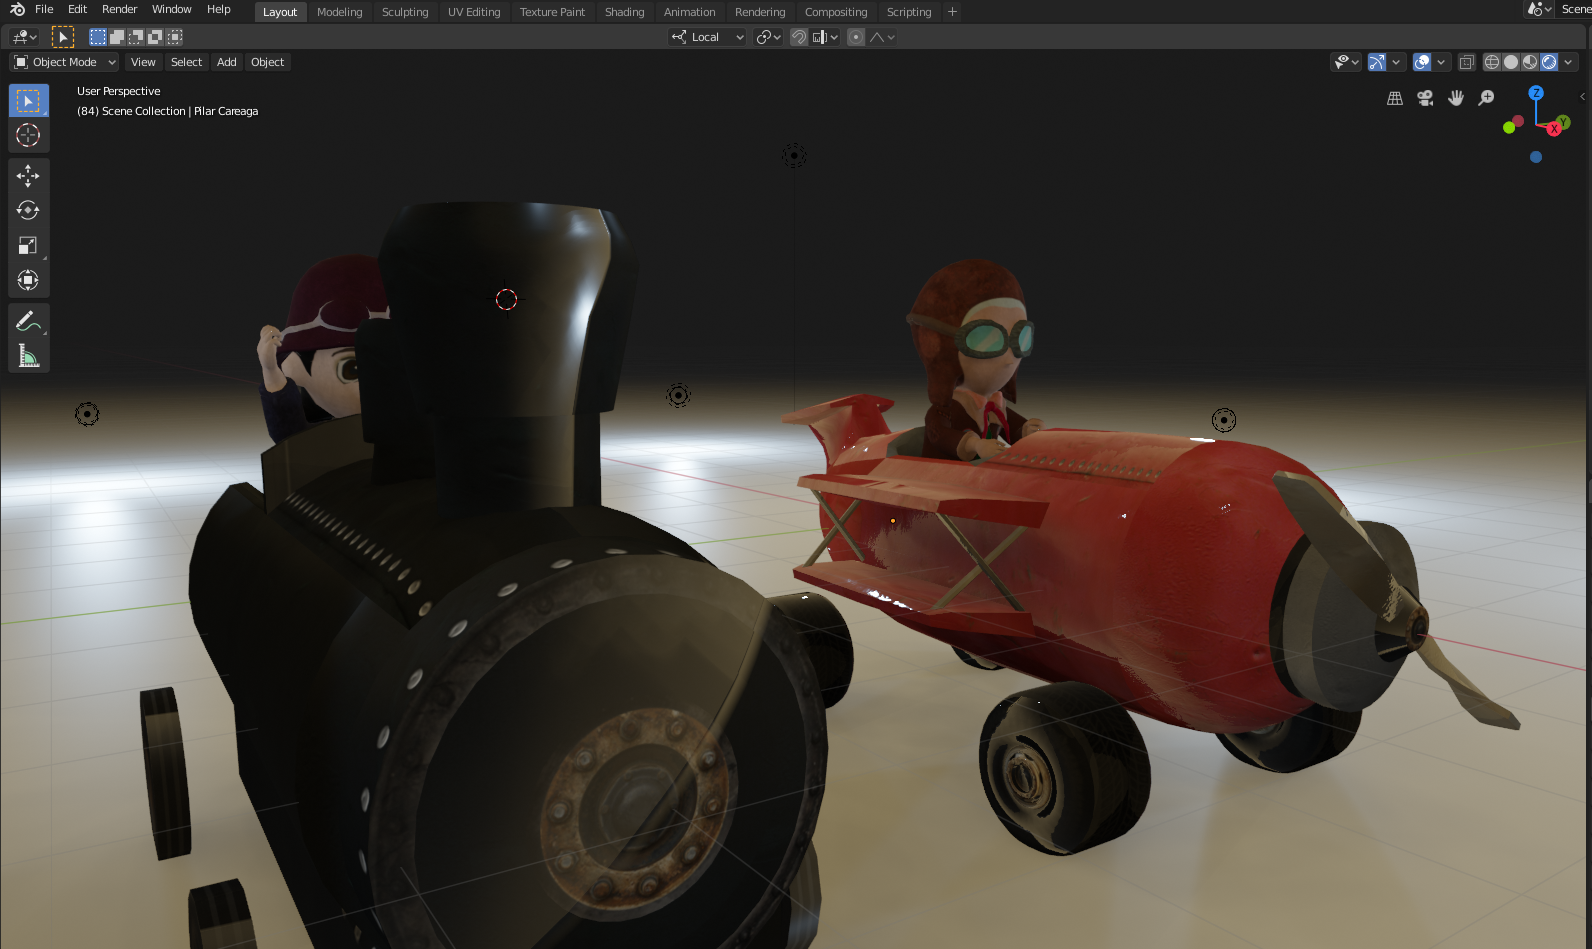
\includegraphics[width=\textwidth]{arte-blender}
	\caption{Modelos de personajes creados en \textit{Blender}.}
	\label{fig:arte-blender}
\end{figure}

\section{Problemas y resolución}

Realizar un videojuego es más complicado de lo que puede aparentar, donde hasta las funciones más simples pueden tener ciertos problemas que ralentizan el correcto transcurso del desarrollo.

Al tratarse de un motor de videojuegos con su propia estructura, las pruebas automáticas no son un aspecto ``amigable'' con esta manera de trabajar, por lo que todas las pruebas realizadas eran manuales y realizadas según fuesen ocurriendo problemas, o bien si surgía una idea a probar.

Estos han sido varios de los problemas surgidos:
\begin{itemize}
\tightlist
	\item Los \textit{meshcolliders} del terreno quitaron un elevado número de horas de trabajo, pues ocasionaban comportamientos imprevistos en el vehículo que, aun configurándolo, impedía el correcto funcionamiento de éste. Al actualizar el mapa a una versión más reciente y con más polígonos, así como añadiendo \textit{colliders} esféricos a las ruedas para que no atravesaran el suelo, se solucionaron gran parte de esos problemas ocasionados.
	\item Las funciones creadas, una vez fueron desarrolladas, funcionaban sin algún tipo de problema. En cambio, cuando se tuvieron que implementar nuevos aspectos, componentes u otros, algunos provocaron fallos inesperados en esas funciones previamente creadas, aparentemente, de manera correcta. Un ejemplo fue el sistema de conteo de vueltas, el cual, al introducir los \textit{colliders} de las ruedas, empezó a realizar un mal conteo provocando la finalización inesperada de la partida al aumentar el número de vueltas completo, lo que hizo necesario un replanteamiento de la lógica de los \textit{scripts} general para que nada empezara a fallar por distintos lados.
	\item Distintos fallos menores solventados en el momento en el que se conocía su existencia.
\end{itemize}

\section{Documentación}

En los inicios del proyecto, se planteó realizar la documentación en documento OpenOffice, pero se vio menos óptimo respecto al tiempo que conlleva formatear el documento que en otras herramientas como LaTeX, de la cual también se tenía plantilla, con lo cual se procedió a comenzar la documentación ahí haciendo uso de Texmaker.

Gracias a esta herramienta se ha podido escribir la documentación centrándose en el contenido con la correcta estructuración de los apartados, índices y elementos gráficos. Los inconvenientes encontrados han sido debidos al desconocimiento del mismo (escritura de algunos caracteres o estructuras erróneas que provocaba una compilación fallida) así como algún fallo menor fácilmente solucionable (reestructurado y reescritura de textos) ralentizando un poco el progreso en las etapas iniciales de la documentación.

\section{Exposición social}

El progreso de este proyecto se ha ido plasmando en las redes sociales de ÍTACA, obteniendo un \textit{feedback} positivo de las personas que han visualizado las publicaciones. Además, se explicó parte de su creación y los problemas a resolver en unas jornadas online organizadas por el mismo Centro el día 16 de junio de 2021, obteniendo también buenas valoraciones y un gran interés por el público \cite{itaca:jornadas}.

\begin{figure}[h]
	\centering
	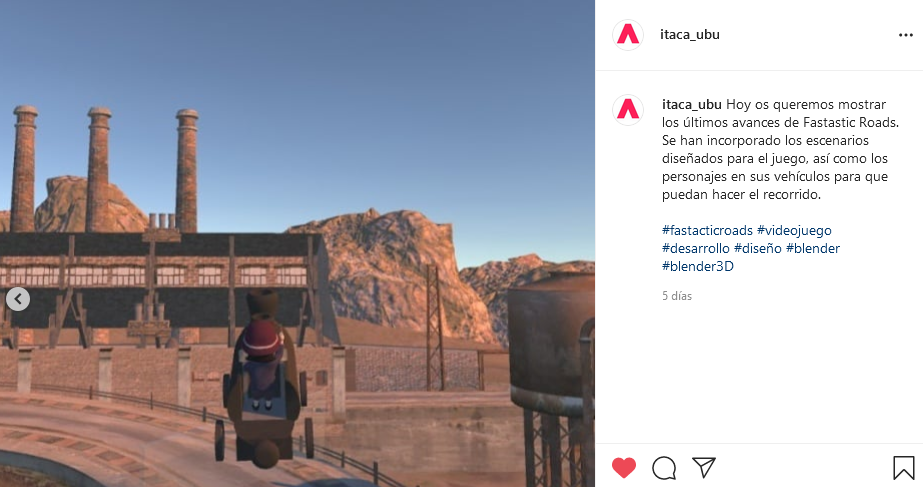
\includegraphics[width=\textwidth]{exposicion}
	\caption{El progreso del proyecto ha podido ser visualizado en Internet.}
	\label{fig:exposicion}
\end{figure}